\begin{problem}[Hatcher {\S}2.1, Ex.\@ 20]
Show that $\widetilde H_n(X)\cong\widetilde H_{n+1}(SX)$ for all $n$, where
$SX$ is the suspension of $X$. More generally, thinking of $SX$ as the
union of two cones $CX$ with their bases identified, compute the reduced
homology groups of the union of any finite number of cones $CX$ with their
bases identified.
\end{problem}
\begin{proof}
First note that the reduced suspension of $X$, $\Sigma X$, which is
homotopy equivalent to $SX$, can be realized as the quotient space
$CX/X$. Given the imbedding $X\hookrightarrow CX$, by 2.16 and excision (or
2.22) we have the long exact sequence in
\begin{equation}
\label{eq:suspension-long-exact-sequence}
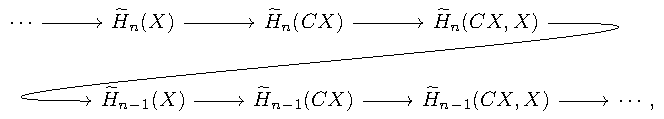
\includegraphics{hw-4-long-exact-sequence-suspension}
\end{equation}
where $\widetilde H_n(CX,X)\cong\widetilde H_n(CX/X)\cong\widetilde
H_n(SX)$. Since $CX$ is contractible, we have $H_n(CX)=0$ for all
$n$ and the long exact sequence \eqref{eq:suspension-long-exact-sequence}
yields an isomorphism
\[
\widetilde H_n(SX)\cong\widetilde H_{n-1}(X).\qedhere
\]
\end{proof}
\newpage

\begin{problem}[Hatcher {\S}2.1, Ex.\@ 22]
Prove by induction on the dimension the following facts about the homology
of a finite dimensional CW complex $X$, using the observation that
$X^n/X^{n-1}$ is a wedge sum of $n$-spheres:
\begin{enumerate}[label=(\alph*)]
\item If $X$ has dimension $n$ then $H_i(X)=0$ for $i>n$ and $H_n(X)$ is
  free.
\item $H_n(X)$ is free with basis in bijective correspondence with the
  $n$-cells if there are no cells of dimension $n-1$ or $n+1$.
\item If $X$ is has $k$ $n$-cells, then $H_n(X)$ is generated by at most
  $k$ elements.
\end{enumerate}
\end{problem}
\begin{proof}
To make Hatcher's comment more precise, if $X=\bigcup_{k=0}^n X^k$ is a
$n$-dimensional CW-complex, by excision the relative homology
\begin{equation}
\label{eq:hw-4-excision-wedgesum-k-spheres}
H_i\left(X^k,X^{k-1}\right)\cong
\widetilde H_i\left(X^k/X^{k-1}\right)
\cong
\widetilde H_i\left(\textstyle{\bigvee_{\alpha_k} S^k}\right)
\cong
\bigoplus_{\alpha_k}\widetilde H_i\left(S^k\right)
\cong
\begin{cases}
\bigoplus_{\alpha_k}\bfZ&\text{if $i=k$}\\
0&\text{otherwise}
\end{cases}
\end{equation}
where $\alpha_k$ is the index over the $k$-dimensional cells of $X$.
\\\\
\textbf{(a)} We proceed by induction on $n$ the dimension of $X$. If $n=0$
then $X^0$ is a collection of points and we know that $H_i(X^0)=0$ for all
$i>0$ and $H_0=\oplus_\alpha\bfZ$ where $\alpha$ runs over all $X^0$.

Now for the inductive step, suppose $H_i(X^{n-1})=0$ for all $i>n-1$. Then,
we have the long exact sequence
\begin{equation}
\label{eq:exact-sequence-induction}
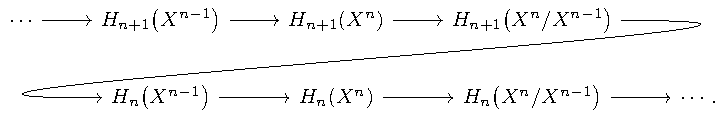
\includegraphics{hw-4-induction-d-cells}
\end{equation}
But by the induction hypothesis, $H_i\left(X^{n-1}\right)=0$ for
all $i>n-1$ and $H_{n-1}\left(X^{n-1}\right)=\bigoplus_\alpha\bfZ$ over
some index $\alpha$. Then \eqref{eq:exact-sequence-induction} becomes
\begin{equation}
\label{eq:hw-4-induction-last}
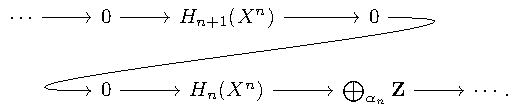
\includegraphics{hw-4-induction-d-cells-filled}
\end{equation}
It's easy to see, if we extend \eqref{eq:hw-4-induction-last} to the left,
i.e., by adding $H_{n+1}$ etc., that $H_i\left(X^n\right)=0$ since it is
sandwiched between two $0$'s. Moreover, by exactness at
$H_n\left(X^n/X^{n-1}\right)$, we have an injection
$H_n\left(X^n\right)\hookrightarrow\bigoplus_{\alpha_n}\bfZ$ so
$H_n\left(X^n\right)$ is free abelian.
\\\\
Now, note that if $m>i$ the $H_i(X)\cong H_i\left(X^m\right)$.
\begin{proof}[Proof of observation]
\renewcommand\qedsymbol{$\clubsuit$}
Since $X$ is $n$-dimensional all we need to show is that
$H_i\left(X^m\right)\cong H_i\left(X^{i+1}\right)$. By induction on $m$,
the base case $m=i+1$ is clear. Now for the inductive step, suppose
$H_i\bigl(X^{m'}\bigr)\cong H_i\left(X^{i+1}\right)$ for $m>i$. Then we
have
\begin{equation}
\label{eq:lemma-1}
\cdots\longrightarrow
H_{i+1}\bigl(X^{m+1},X^m\bigr)\longrightarrow
H_i\bigl(X^m\bigr)\longrightarrow
H_i\bigl(X^{m+1}\bigr)\longrightarrow
H_i\bigl(X^{m+1},X^m\bigr)\longrightarrow
\cdots.
\end{equation}
But $H_{i+1}\bigl(X^{m+1},X^m\bigr)\cong
H_{i+1}\bigl(X^{m+1},X^m\bigr)\cong 0$ so $H_i\bigl(X^m\bigr)\cong
H_i\bigl(X^{m+1}\bigr)$, as desired.
\end{proof}
\textbf{(b)} If $n<1$ in the case $n=0$ there are no $1$-cells and in the
case $n=1$ there are no $0$-cells so we cannot say anything. Therefore, we
begin at $n>1$. By our observation, we have $H_n(X)\cong H_n(X^n)$ and by
part \textbf{(a)} we have
\begin{equation}
  \label{eq:short-exact-cells}
\cdots\longrightarrow
H_n\bigl(X^{n-2}\bigr)\longrightarrow
H_n\bigl(X^n\bigr)\longrightarrow
H_n\bigl(X^n,X^{n-2}\bigr)\longrightarrow
H_{n-1}\bigl(X^{n-2}\bigr)\longrightarrow
\cdots,
\end{equation}
where $H_n\left(X^{n-2}\right)\cong H_{n-1}\left(X^{n-2}\right)\cong
0$. Hence, by exactness at $H_n\left(X^n\right)$, we have
$H_n\left(X^n\right)\cong H_n\left(X^n,X^{n-2}\right)$ so by 2.34 (a), we
have
\[
H_n\left(X^n\right)\cong
H_n\left(X^n,X^{n-1}\right)\cong
H_n\left(X^n,X^{n-2}\right)\cong\bigoplus_\alpha\bfZ
\]
where $\alpha$ is an index over the $n$-cells of $X$.
\\\\
\textbf{(c)} By the observation $H_n(X)\cong
H_n\left(X^{n+1}\right)$. Moreover, we have the following exact sequence
\begin{equation}
  \label{eq:short-exact-cells-2}
\cdots\longrightarrow
H_n\left(X^{n+1},X^n\right)\longrightarrow
H_n\left(X^n\right)\longrightarrow
H_n\left(X^{n+1}\right)\longrightarrow
H_n\left(X^{n+1},X^n\right)\longrightarrow\cdots
\end{equation}
where $H_{n+1}\left(X^{n+1},X^n\right)\cong
H_n\left(X^{n+1},X^n\right)\cong 0$ giving us an injection
$H_n\left(X^n\right)\hookrightarrow H_n\left(X^{n+1}\right)$. By part
\textbf{(a)}, $H_n\left(X^n\right)$ is free abelian and has rank at most
the the number of $n$-cells of $X$. Thus, $H_n\left(X\right)$ is free abelian
and has rank at most the number of $n$-cells of $X$.
\end{proof}
\newpage

\begin{problem}[Hatcher {\S}2.2, Ex.\@ 2]
Given a map $f\colon S^{2n}\to S^{2n}$, show that there is some point $x\in
S^{2n}$ with either $f(x)=x$ or $f(x)=-x$. Deduce that every map
$\bfRP^{2n}\to\bfRP^{2n}$ has a fixed point. Construct maps
$\bfRP^{2n-1}\to\bfRP^{2n-1}$ without fixed points from linear
transformations $\bfR^{2n}\to\bfR^{2n}$ without eigenvectors.
\end{problem}
\begin{proof}
Given a map $f\colon S^{2n}\to S^{2n}$, either $f$ has a fixed point or it
does not. If $f$ does not have a fixed point then $f\simeq a$ so $\deg
f=(-1)^{2n+1}=-1$ so $\deg(-f)=\deg(-\Id\circ f)=1$ has a fixed point for
otherwise we may homotope $f$  to the antipodal map $a$ and so, by
transitivity, $\Id\simeq a$, but this is nonsense.

Realize $\bfRP^{2n}$ as the quotient $S^{2n}/\sim$ where $x\sim -x$.

Note that $p\colon S^{2n}\to\bfR^{2n}$ is a cover of $\bfR^{2n}$.
Let $f\colon\bfRP^{2n}\to\bfRP^{2n}$. By
\end{proof}

%%% Local Variables:
%%% mode: latex
%%% TeX-master: "../MA572-HW-Current"
%%% End:
